\subsection{Che cos'è un LLM}

Un \emph{large language model} è, nella sua forma più diffusa, una rete neurale basata sull'architettura
\emph{Transformer} \cite{vaswani2017attention}, addestrata a predire il token successivo di una sequenza di testo a partire dai token che lo precedono. L'elemento che ha reso questa architettura dominante rispetto ai modelli ricorrenti che la precedevano è il meccanismo di \emph{self-attention}: ogni token della sequenza viene messo in relazione diretta con tutti gli altri, indipendentemente dalla loro distanza, e questo permette al modello di catturare dipendenze a lungo raggio nel testo senza il collo di bottiglia sequenziale delle reti ricorrenti. Soprattutto, la self-attention rende l'addestramento parallelizzabile su hardware specializzato, una condizione necessaria per scalare questi modelli alle dimensioni che oggi li caratterizzano, sia in termini di parametri sia di dati di addestramento.

% ---------------------------------------------------------------------------
% Tokenizzazione
% ---------------------------------------------------------------------------
Prima di poter essere elaborato da un LLM, il testo deve essere convertito in una sequenza di unità discrete, i \emph{token}. Un token non coincide necessariamente con una parola: le parole più frequenti corrispondono in genere a un singolo token, mentre quelle meno comuni vengono spezzate in più frammenti sub-lessicali, fino ad arrivare, nei casi limite, ai singoli caratteri. La segmentazione è stabilita da un \emph{tokenizer}, un algoritmo che apprende da un corpus di riferimento quali frammenti di testo ricorrono più spesso. Il più diffuso, il \emph{Byte-Pair Encoding} (BPE), parte dai singoli caratteri e fonde iterativamente le coppie di simboli adiacenti più frequenti, fino a costruire un vocabolario di dimensione prefissata, tipicamente dell'ordine di decine o centinaia di migliaia di token. Come illustra la Figura~\ref{fig:tokenizzazione}, a ogni token del vocabolario è associato un identificativo numerico, ed è questa sequenza di numeri, e non il testo, che il modello riceve in ingresso e produce in uscita. In questo modo un vocabolario finito è sufficiente a rappresentare qualunque testo, comprese parole mai incontrate durante l'addestramento.

La tokenizzazione ha una conseguenza pratica diretta: tutte le grandezze che caratterizzano un LLM sono misurate in token, non in parole o in caratteri. In particolare, la \emph{finestra di contesto}, ovvero il numero massimo di token che il modello può elaborare in un'unica interazione, prompt e risposta compresi, va da poche migliaia a centinaia di migliaia di token a seconda del modello, e pone un limite diretto alla quantità di testo recuperato (Sezione~\ref{sec:rag}) che può essere fornita come contesto per una singola domanda. Il numero di token necessari a rappresentare uno stesso contenuto, inoltre, varia da una lingua all'altra: Petrov et al. \cite{petrov2023unfairness} mostrano che i tokenizer, addestrati su corpus in cui l'inglese è prevalente, segmentano in genere le altre lingue in un numero maggiore di token. A parità di contenuto, quindi, un documento in italiano può occupare una porzione della finestra di contesto più ampia del suo equivalente in inglese.

\begin{figure}[H]
  \centering
  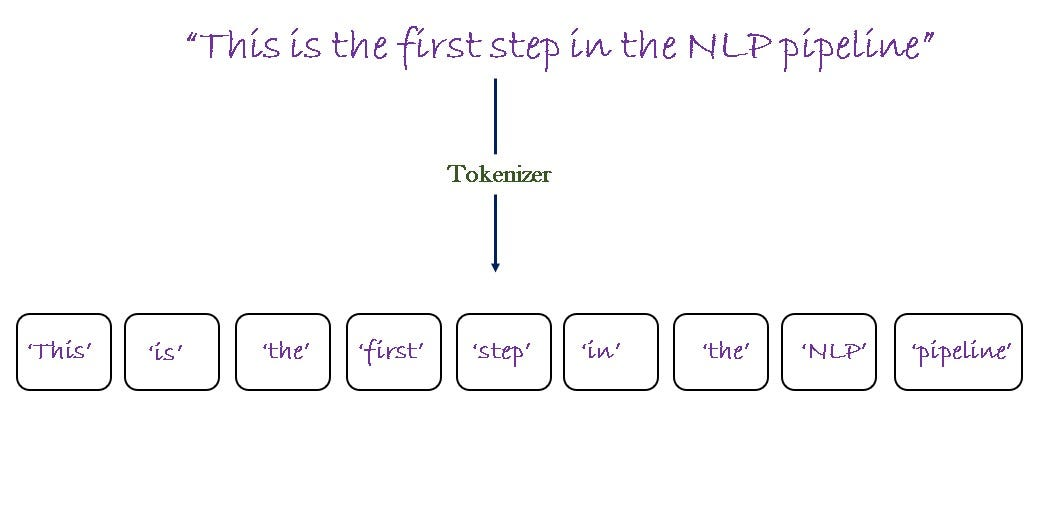
\includegraphics[width=0.99\textwidth]{assets/tokenizer.jpg}
  \caption{Tokenizzazione di una domanda in linguaggio naturale. Il tokenizer segmenta il testo in token. A ciascun token è associato un
    identificativo intero $i_k$ nel vocabolario del modello. La segmentazione mostrata è a scopo illustrativo:
    quella effettiva dipende dal tokenizer del modello considerato.}
  \label{fig:tokenizzazione}
\end{figure}

% ---------------------------------------------------------------------------
% Generazione auto-regressiva
% ---------------------------------------------------------------------------
In fase di generazione, i LLM operano in modo \emph{auto-regressivo}. Data una sequenza di token $x_1, \dots, x_t$, il modello calcola una distribuzione di probabilità sull'intero vocabolario per il token successivo, $P(x_{t+1} \mid x_1, \dots, x_t)$; da questa distribuzione viene scelto un token, il più probabile oppure uno campionato secondo la strategia di \emph{decoding} adottata, che viene accodato alla sequenza e diventa a sua volta parte del contesto per il passo seguente. Il procedimento si ripete un token alla volta, finché il modello non produce un token speciale di fine sequenza o non raggiunge un limite di lunghezza prefissato. La probabilità di un'intera sequenza si scompone quindi nel prodotto delle probabilità di ciascun token, condizionate ai token che lo precedono:
\begin{equation}
  P(x_1, \dots, x_T) = \prod_{t=1}^{T} P(x_t \mid x_1, \dots, x_{t-1}).
  \label{eq:autoregressivo}
\end{equation}
Nell'architettura Transformer questo vincolo è imposto da una \emph{maschera causale} applicata alla self-attention, che impedisce a ciascun token di considerare quelli che lo seguono. Per questo motivo i LLM generativi adottano in genere la variante \emph{decoder-only} dell'architettura, a differenza di modelli come BERT, che osservano l'intera sequenza in entrambe le direzioni e non sono pensati per generare testo. La maschera causale spiega anche perché addestramento e generazione abbiano costi così diversi: in addestramento, la sequenza è nota per intero e il modello può calcolare in parallelo le previsioni per tutte le posizioni; in generazione, invece, ogni token dipende da quelli prodotti in precedenza, e il processo è intrinsecamente sequenziale. Ne derivano due conseguenze rilevanti per questo lavoro. La prima riguarda i tempi di risposta, che crescono con la lunghezza del testo generato oltre che con quella del contesto fornito. La seconda riguarda l'affidabilità: il modello non produce la risposta nel suo insieme né rivede quanto ha già scritto, ma sceglie a ogni passo una continuazione plausibile del testo; un token errato entra nel contesto e condiziona tutti i successivi, e il campionamento introduce la componente stocastica richiamata nella Sezione~\ref{sec:problema}.

% ---------------------------------------------------------------------------
% Le tre fasi dell'addestramento
% ---------------------------------------------------------------------------
L'addestramento di un LLM avviene tipicamente in tre fasi successive, illustrate nella Figura~\ref{fig:llm-training}. Nella prima, il \emph{pre-training}, il modello
viene esposto a un corpus testuale di dimensioni enormi --- miliardi o migliaia di miliardi di token raccolti dal web, da libri, da codice sorgente --- con il solo obiettivo di predire il token successivo. Questa fase, auto-supervisionata e quindi priva di etichette fornite da esseri umani, fa emergere la competenza linguistica e una parte significativa della conoscenza fattuale del modello, codificata implicitamente nei suoi parametri \cite{zhao2023survey}.
Un modello che ha completato solo questa fase, tuttavia, non è ancora un assistente conversazionale: è un sistema di completamento testuale, che tende a proseguire il prompt ricevuto piuttosto che a rispondere a una domanda. La seconda fase, l'\emph{instruction-tuning}, affina il modello pre-addestrato in modo supervisionato su coppie istruzione-risposta scritte da esseri umani, insegnandogli a seguire le istruzioni ricevute e a rispondere nella forma attesa.

La terza fase, l'\emph{allineamento}, adatta ulteriormente il comportamento del modello alle preferenze umane, tipicamente tramite \emph{reinforcement learning from human feedback} (RLHF). Come mostra la parte inferiore della Figura~\ref{fig:llm-training}, questa fase si articola in due passaggi: prima si addestra un modello di ricompensa (\emph{reward model}) su confronti tra risposte alternative, ordinate per qualità da annotatori umani; poi si aggiorna iterativamente il modello linguistico con tecniche di apprendimento per rinforzo, usando come segnale la ricompensa stimata da quel modello. Ouyang et al. \cite{ouyang2022instructgpt}, nel lavoro che ha introdotto InstructGPT, mostrano che le ultime due fasi contano non meno della scala del modello nel renderlo utile e sicuro dal punto di vista comportamentale: un modello InstructGPT da 1,3 miliardi di parametri, sottoposto a instruction-tuning e RLHF, viene preferito dai valutatori umani a un modello GPT-3 da 175 miliardi di parametri privo di questo affinamento.

Sono quindi la seconda e la terza fase a rendere un LLM capace di rispondere in modo pertinente nella forma a una domanda posta in linguaggio naturale. Il modello resta però, come discusso nella Sezione~\ref{sec:problema}, incapace di garantire che il contenuto della risposta sia corretto o aggiornato. Né l'instruction-tuning né l'allineamento affrontano questo limite, perché esso riguarda la conoscenza codificata nei parametri e non il comportamento del modello: la conoscenza fattuale si forma quasi interamente nel pre-training, mentre le fasi successive modificano il comportamento del modello senza aggiungere, se non marginalmente, nuova conoscenza.

\begin{figure}[H]
  \centering
  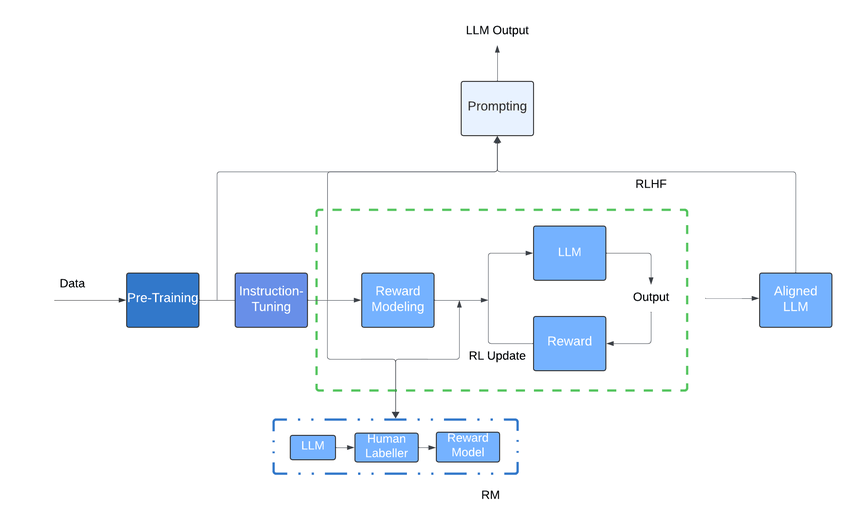
\includegraphics[width=0.9\textwidth]{assets/A-basic-flow-diagram-depicting-various-stages-of-LLMs-from-pre-training-to.png}
  \caption{Le fasi che portano dai dati grezzi a un LLM allineato e utilizzabile tramite prompting: pre-training,
    instruction-tuning e, infine, l'allineamento tramite \emph{reward modeling} (RM, in basso: un modello di
    ricompensa addestrato su confronti prodotti da annotatori umani) e \emph{reinforcement learning from human
    feedback} (RLHF, al centro: un ciclo iterativo che aggiorna l'LLM in base al segnale del modello di ricompensa).}
  \label{fig:llm-training}
\end{figure}

% ---------------------------------------------------------------------------
% Leggi di scala
% ---------------------------------------------------------------------------
Un altro aspetto, rilevante per la scelta dei modelli discussa nella sezione seguente, è il legame tra le dimensioni di un modello e la qualità delle sue previsioni. Kaplan et al. \cite{kaplan2020scaling} hanno misurato sperimentalmente come varia l'errore di predizione di un modello linguistico, cioè quanto spesso e quanto nettamente il modello sbaglia nel prevedere il token successivo, al variare di tre fattori: il numero di parametri del modello, la quantità di dati usati per addestrarlo e la potenza di calcolo complessivamente impiegata. Il risultato è una relazione sorprendentemente regolare, detta \emph{legge di scala} (\emph{scaling law}): finché gli altri due fattori non fanno da collo di bottiglia, l'errore diminuisce secondo una legge di potenza al crescere di ciascun fattore. In termini intuitivi, moltiplicare un fattore per una stessa quantità produce sempre lo stesso miglioramento in termini relativi. Secondo le stime degli autori, per esempio, raddoppiare il numero di parametri riduce l'errore di circa il 5\%, sia che si passi da 10 a 20 milioni di parametri, sia che si passi da 500 milioni a un miliardo. La Figura~\ref{fig:scaling} mostra questo andamento: su assi in scala logaritmica, le tre relazioni appaiono come rette discendenti.

Ne derivano due conseguenze. La prima è che un modello più grande, a parità di architettura e di dati di addestramento, è in genere più capace: è questa relazione, osservata ancor prima della diffusione dei moderni LLM conversazionali, a motivare l'esistenza di famiglie di modelli disponibili in più taglie, come Qwen2.5-7B e Qwen2.5-14B discussi nella sezione seguente. La seconda è che ogni ulteriore miglioramento costa sempre di più in termini assoluti: per ridurre l'errore di un'altra frazione fissa occorre ogni volta moltiplicare le risorse, e il modello più grande richiede più memoria e più tempo di calcolo per ogni risposta generata e per il training. La scelta della taglia è quindi un compromesso tra qualità delle risposte e risorse disponibili.

\begin{figure}[H]
  \centering
  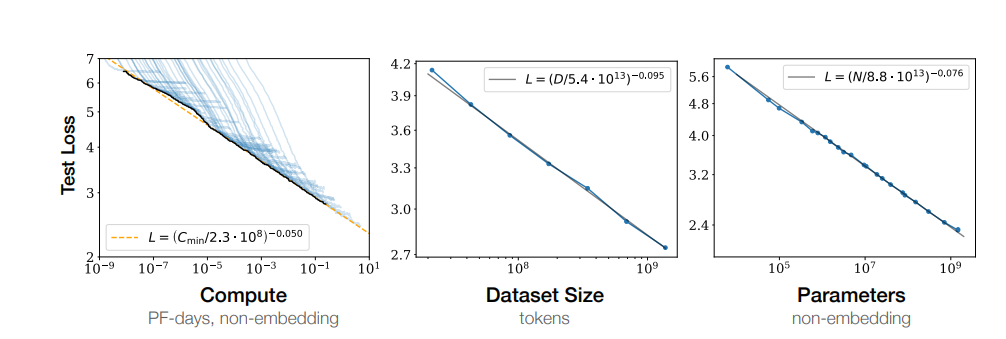
\includegraphics[width=0.9\textwidth]{assets/scale_law.png}
  \caption{Le prestazioni del modello linguistico migliorano in modo continuo man mano che aumentiamo la dimensione del modello, la dimensione del dataset e la quantità di calcolo usata per l'addestramento. Per ottenere prestazioni ottimali, tutti e tre i fattori devono essere aumentati insieme. Fonte: Kaplan et al. \cite{kaplan2020scaling}}
  \label{fig:scaling}
\end{figure}


% ---------------------------------------------------------------------------
% In-context learning
% ---------------------------------------------------------------------------
Al crescere della scala emerge anche una capacità che non corrisponde a una specifica fase di addestramento, ma che è rilevante per inquadrare il
funzionamento di un sistema RAG come quello di questo lavoro: l'\emph{in-context learning}. Brown et al.
\cite{brown2020gpt3}, presentando GPT-3, osservano che un modello linguistico sufficientemente grande può adattare il proprio comportamento a un compito nuovo semplicemente a partire da istruzioni o esempi forniti nel testo del prompt, senza alcun aggiornamento dei suoi parametri. È precisamente questo meccanismo, e non un nuovo addestramento, che un sistema RAG sfrutta quando fornisce al modello un contesto recuperato al momento della domanda (Sezione~\ref{sec:rag}): il modello non apprende un fatto nuovo in modo permanente, ma lo usa temporaneamente, limitatamente alla singola interazione in cui compare nel prompt.

% ---------------------------------------------------------------------------
% Closed-weight vs open-weight
% ---------------------------------------------------------------------------
Ai fini di questo lavoro è rilevante, infine, la distinzione tra modelli \emph{closed-weight}, accessibili solo tramite
un'interfaccia remota gestita dal fornitore e generalmente a pagamento, e modelli \emph{open-weight}, i cui parametri sono
pubblicati e possono essere eseguiti su hardware proprio. La scelta di adottare esclusivamente modelli open-weight risponde a due esigenze. La prima è il contenimento dei costi: i servizi closed-weight sono tipicamente tariffati in base al numero di token elaborati, per cui la spesa cresce con il numero di domande ricevute ed è difficile da prevedere per un servizio rivolto a un'intera università; un modello eseguito in locale comporta invece un costo legato essenzialmente all'hardware e al suo funzionamento, indipendente dal volume di utilizzo. La seconda è la tutela delle informazioni dell'ateneo: con un modello closed-weight, a ogni interrogazione la domanda dello studente e i documenti recuperati per rispondere verrebbero inviati a un fornitore esterno, mentre l'esecuzione in locale permette di non affidare a terzi documenti, contenuti del sito e informazioni proprietarie. Per questi motivi, tutti i modelli generativi considerati in
questo lavoro, descritti nella sezione seguente, sono modelli open-weight eseguibili interamente in locale.